%\documentstyle{llncs}
%\documentclass[12pt,fullpage]{llncs}
\documentclass[12pt]{article}
%\usepackage[left=3cm,top=1.2cm,right=3cm,nohead,nofoot]{geometry}
%\usepackage[letter,left=.25in,right=.25in,top=.17in,textwidth=7.5in,textheight=9in]{geometry}
%\usepackage[left=0cm]{geometry}

%\documentclass[12pt]{report}
%\usepackage {utthesis2}              %% Preamble.

%\usepackage{amsmath}
%\usepackage{amssymb}
\usepackage{arabtex}
\usepackage{amsmath}
\usepackage{amssymb}
\usepackage{times}
\usepackage{caption}
\usepackage{epsfig}
\usepackage{subfigure}
\usepackage{color}
\usepackage{rotate}
\usepackage{rotating}
\usepackage{multirow}
%\usepackage[colorlinks=false]{color,hyperref}
\usepackage{color,hyperref}
%\usepackage{amsthm}
\usepackage{booktabs}
\usepackage{multirow}
\usepackage{natbib}
\bibpunct{[}{]}{,}{n}{}{;}

\usepackage{url}

\usepackage{relsize}
\usepackage{fancyvrb}
\usepackage{fancyhdr,lastpage}

\usepackage{utf8}
\setarab
\fullvocalize
\transtrue
\arabtrue

\newcommand{\CharCodeIn}[1]{`\CodeIn{#1}'}
\newcommand{\CodeIn}[1]{{\small\texttt{#1}}}
\newcommand{\frl}[1]{\fbox{\RL{#1}}} 
\newcommand{\noArRL}[1]{\arabfalse\RL{#1}\arabtrue} 
\newcommand{\noTrRL}[1]{\transfalse\RL{#1}\transtrue} 
\newcommand{\noTrNoVocRL}[1]{\novocalize\transfalse\RL{#1}\transtrue\vocalize} 
%\newcommand{\drawline}{\begin{picture}(6,.1) \put(0,0) {\line(1,0){6.25}}\end{picture}}

\usepackage{setspace}
%\doublespacing
\renewcommand{\baselinestretch}{1.15}
\setlength{\parindent}{0in}
%\parskip 6pt
%\parindent 0pt
%\setlength{\parskip}{.05in}
%\oddsidemargin 0in
%\evensidemargin 0in
\oddsidemargin .0in
\evensidemargin .0in
\hoffset -.75in
\voffset -.83in
\textwidth 7.5in
\textheight 9.5in

\topsep 0in
\topmargin 0.17in

%\usepackage{arabtex}
%\usepackage{utf8}

\begin{document}


\pagestyle{fancy}
%\lhead{}
\chead{}
\rhead{NPRP No.~:~~~~4-484-1-075}

\lfoot{QNRF Form}
\cfoot{}
\rfoot{Page \thepage~of~\pageref{LastPage} }
\renewcommand{\footrulewidth}{0.2pt}
\renewcommand{\headrulewidth}{0.2pt}

%\begin{titlepage}

\begin{center}
{\Large \bf Relational Arabic Text Mining Framework using 
    Morphological
    and Case-Based Analysis }

%\setlength{\unitlength}{1in}
%\setlength{\unitlength}{1in}
\vspace{1.5in}

\renewcommand{\arraystretch}{.6}
\begin{tabular}{cc}
Fadi Zaraket & Rehab Duwairi \\
Electrical and Computer Engineering &  Computer Science and Engineering Department \\
American University of Beirut & University of Qatar \\
{\tt fadi.zaraket@aub.edu.lb} & {\tt Rehab.Duwairi@qu.edu.qa}
\end{tabular}

\vspace{1.5in}

\renewcommand{\arraystretch}{.6}
\begin{tabular}{c}
{\small Research Plan Document } \\
{\small Proposal Submitted to }\\
\\
    Qatar National Research Foundation \\
    National Priorities Research Program \\
    4$^{th}$ Cycle 
\end{tabular}
\vspace{.5in}

\date{\today}
\pagebreak

\end{center}

\section{Background (max of 2 pages)}
\label{s:background}

Research in text mining started in the mid 1980s when Swanson 
realized that slicing and combining seemingly unrelated medical 
articles led to the discovery of new 
hypotheses~\cite{JNi06}.
Till present, most of the interest in text mining comes 
from biological sciences.
Lately we saw applications of text mining in the advertisement, 
political campaigning, and other businesses.
Text mining involves information retrieval (IR), natural language 
processing (NLP), information extraction (IE), 
and data mining~\cite{ASr09}.

The almost comprehensive book 
``Arabic Computational Morphology''~\cite{Sou07}
covers most academic research work on Arabic text mining.
It summarizes recent work, and presents strong evidence of 
shortage of historic research. It also highlights  an emerging 
interest with a specific application to machine 
translation from Arabic to English after 2001.
The research community showed little interest in 
automating Arabic text analysis that may serve
the Arabic user.
While machine translation is of general interest, 
an Arabic user is more interested in 
information hard to discover manually.
Examples are the relation between clinical records, pharmaceutical 
prescriptions and sales, and a specific sickness,
the relation
between stock prices and political news, or the 
relation between interrogation reports with suspects
and investigative reports from the crime scenes. 

We propose to build a framework for
%{\em relational text mining 
%of Arabic using morphological and case-based analysis}. 
{\em case-based Arabic text analysis using relations and morphology} (CATARM). 
CATARM will apply novel algorithms and tools
to answer queries seeking relations amongst
Arabic text documents.
CATARM takes as input several sets of documents, each of a specific
type, and a user query. % expressed in a visual language.
The query, expressed in a visual language, allows the user 
to build a flow of Arabic text mining
components and discover desired relations between documents. 
CATARM compiles the query into a netlist of computational 
components. It also uses features extracted from the query and 
the document sets to simplify the computational 
components. 
%The main CATRAM computational components will be finite 
%state machines (FSM) that express a linguistic model of the Arabic 
%language and that can be parametrized and relaxed to fit a case 
%study. 

\novocalize
%The accuracy of the solutions suffer due to inherent difficulties
%of morphological analysis of the Arabic language. 
It is common practice to write Arabic text
without short vowels. 
This greatly increases the ambiguity of Arabic text. 
Arabic letters can have up to 
four different forms
corresponding to their position in a word, i.e. beginning,
middle, end of word and separate forms. 
This allows the phrase
\noTrRL{il_A\nospace almdrsT}  with no delimiter within
to be visually recognizable
as two separate words \RL{il_A} (to) and \RL{almdrsT} (the school).
This happens because the first word \RL{il_A} ends with
\RL{_A} a non-connecting letter. 
These words occur often in text and greatly increase the
difficulty of tokenization and are referred to as 
``run-on'' words~\cite{Buckwalter:04}.
Such difficulties are inherent to the 
morphological analysis of the Arabic language and
render the solutions inaccurate.


Arabic morphological analyzers~\cite{Sughaiyer:04}
consider an Arabic word and its internal structure composed of 
several {\em morphemes}. 
A morpheme is a {\em stem} or an {\em affix}.
An affix is a {\em prefix, suffix,} or an {\em infix}.
The analysis of one word may lead to several possible
solutions.
\vocalize
For instance, the word 
\RL{'a.hmadH}~\footnote{In this document, we use the default 
ArabTeX transliteration style ZDMG.}
may have two valid morphological analyses. 
The word means ``I praise him'' when
the letter \RL{'a} is a prefix and  it means
``his Ahmad'' when 
the letter \RL{'a} is part of the proper noun stem 
\RL{'a.hmad}.
\novocalize

Current morphological analyzers such as 
Buckwalter~\cite{Buckwalter:02},
Beesley~\cite{Beesley:01}, SAMA~\cite{Kulick:10},
and ElixirFM~\cite{Otakar:07} exist
and are used in several open source spell checkers as 
well as NLP frameworks~\cite{Col09}.
They take as input white space delimited tokens~\cite{Kulick:10},
consider them as words,
and enumerate all possible solutions. 
This approach has several problems. 
First, a white space delimited token may have 
more than one word.
Second, the exhaustive enumeration may hurt performance and may
not be necessary or appropriate
in some case studies~\cite{Maamouri:10}. 
Other morphological analyzers such as 
Amira~\cite{Diab:07,Benajiba:07},
MAGEAD~\cite{Habash:05}, and MADA+TOKAN~\cite{Habash:09} 
use machine learning and support vector machines (SVM) 
to enhance the accuracy at the expense of efficiency.

{\bf Hypothesis 1.} We hypothesize that many case studies, 
in particular relational ones, 
do not require high accuracy from the 
low level morphological analysis.
The sophistication of the higher level query can eliminate 
many ambiguous low level solutions at a lower computational 
cost.
For example, if a query concerns proper names and the 
prefix in question in the analysis connects only to a verb, 
we no further need to analyze the rest of the word.

We find evidence to our hypothesis in~\cite{Maamouri:10} where 
a new corpus was added to the Arabic Tree Bank 
(ATB)~\cite{Maamouri:04}. 
The addition required compliance with the DARPA GALE program 
including several NLP tasks such as English translation 
annotations and word-level alignment of Arabic and English. 
The new genre of data challenged the existing data processing and 
annotation guidelines. 
Alternative guidelines came to place where the high level NLP 
task interacted with the morphological analyzer. 
This led to refining SAMA~\cite{Kulick:10}. 
The work of Habash~\cite{Habash:06} reports that different 
types of morphological analyses behave differently on the same case 
study. 
For one, the analyzers may find different solutions. 
The analyzers may present the solutions in different orders. 
The presented solutions and the order of presentation may not be 
appropriate for the case study. 
We find strong evidence in our preliminary results 
that a case-based morphological analyzer that allows a case-based 
controller to intervene at every decision to guide, use, order, and 
refine the morphological analysis is of high utility.


%Prior work in Arabic text mining addressed the classification and 
%categorization of Arabic text and made little use of features 
%unique to the Arabic language.
Researchers in~\cite{AEL07,Ham07,Abd07,MEl03} 
preprocessed the Arabic text and presented it to known 
techniques that tend to Latin text and queries.
%Buckwalter~\cite{Bee89,Tim04} uses morphological analysis to enable 
%relaxed stemming of Arabic words.
El-Halees used statistical analysis to address the problem of 
classifying Arabic text documents with maximum 
entropy~\cite{AEL07}.
In~\cite{Abd07} Mesleh evaluated six different techniques to 
classify Arabic text using a support vector machine.
El Dost~\cite{MEl03} used root words in the Arabic language to 
speed up automated and hierarchical indexing.
Al-Zoghby~\cite{Ham07}
%addresses the problem of 
%entities extracted from Arabic text with similar content but 
%slightly different names via 
used the derivation feature in 
the Arabic language as a similarity measurement.
%This work is limited to the names of the fields in the data 
%structures extracted from Arabic texts.

{\bf Hypothesis 2.} 
The preprocessing approach does not tend directly to 
the Arabic users who write their 
queries in Arabic and think in Arabic.
We hypothesize that Arabic queries use rules and 
look for relations similar in nature to the structure of the Arabic language 
and the text under investigation.
Thus techniques native to the Arabic language will do better 
in Arabic text analysis.

The work of the CADIM \noTrRL{q-adim} 
project~\cite{Col09} at the University of Columbia supports our 
hypothesis. They observe that Arabic texts used as training 
data for common NLP techniques proved ineffective. 
They built semi-automatic models to address the problem of
Arabic speech recognition.


%\subsection{\bf Arabic text mining in industry}
Few companies in the industry provide Arabic text 
analysis tools.
Sakhr~\cite{Sak09} provides a categorization 
tool with a limited number of predefined categories.
Sakhr also provides a summary 
generator that selects important sentences from text.
Basis technology~\cite{Bas09} provides Rosette, a lexical 
analysis tool that normalizes Arabic text as a pre-processing step 
for general purpose data mining 
tools.  Basis also provides REX; an entity extractor.

ElixirFM~\cite{Otakar:07} uses an {\em inferential-realizational}
approach for morphological analysis
and considers the form of the word 
\noTrRL{.sarf}  instead of its segments. 
Formal rules express the relations between 
the root of the lexeme and the fully inflected word. 
While the rules capture features unique to the 
the Arabic language and its linguistic description~\cite{Badawi:04},
the approach is computationally expensive and enumerates 
all the possible solutions. 

{\bf Goals.} 
CATARM tends to relational Arabic text mining using 
{\bf (1.)} a novel case-based morphological analyzer.
{\bf (2.)} CATARM will build a novel and efficient 
linguistic computational model (LCM) for Arabic. 
%The LCM will be implemented using efficient structures. 
The LCM will be amenable to novel 
{\bf (3.)} Arabic specific simplifications 
inferred from the correspondence between the formal Arabic rules
and the user queries, and 
{\bf (4.)} language independent simplifications
inferred from statistical features %extracted from the documents 
using language independent techniques such as 
hidden Markov models (HMM)~\cite{JanHMM06}
and latent semantic indexing (LSI)~\cite{LSI89}.
%CATARM will augment current digital dictionaries to resolve 
%entity semantics and targeted qualificationsl.
{\bf (5.)} CATARM extracts semantic graphs 
and uses set arithmetic and graph analysis techniques
to establish relations between the graphs. 
{\bf (6.)} CATARM will solve the case studies 
presented in Sections~\ref{s:design:lit}--\ref{s:design:med}.

\pagebreak

\section{Objectives and significance (max of 1 page) } 
\label{s:objectives}

The current prevailing direction in research 
in Arabic text mining and NLP focuses on machine translation from 
Arabic to English. 
A little attention is given to native Arabic text mining 
problems and applications. 
CATARM is a relational Arabic text mining 
framework that tends to Arabic users 
with the following objectives.

\begin{itemize}\itemsep0pt
\item CATARM will build a formal Arabic computational model
using efficient and configurable data structures such as 
finite state machines (FSM). 
\item CATARM will provide the user with a visual query 
language that makes it easy to enter relational queries. 
The query language will also allow the framework to extract Arabic
specific features from the query to simplify the linguistic 
computational model. 
\item CATARM will use statistical models and techniques
to infer language independent features from the text documents
that will further simplify the computational model. 
\item During the project, we will augment current Arabic digital 
dictionaries to resolve entity semantics and targeted 
qualifications such as adjectives.
\item The framework will allow the integration of library and 
custom computational components built on top of primitive
CATARM components. 
The components will be the linguistic computational model,
statistical, set arithmetic, logic,
and graph analysis techniques, and  text algorithms.
\item We will use CATARM to solve several realistic case studies.
We will look at the hadith literature and build a system using
CATARM to relate the hadith literature to the biographies of the
narrators and extract an authenticity graph for the narrators.
We will look at investigation and interrogation security reports
and build a CATARM system that looks for relations between suspects
in the reports. 
We will look at clinical reports and relate them to pharmaceutical 
records and find relations between sicknesses and prescribed medication. 
Finally, we will use CATARM to provide content-based parental control
for Arabic text documents. We will look for 
relations between documents requested by a minor and
a set of undesired Arabic documents. 
If the relation is strong, we will flag access to
the documents. 

We further explain our approach with examples and discuss 
how we will obtain the documents 
in Sections~\ref{s:design:lit}--\ref{s:design:med}.
We will generalize all components built during the development 
of the case studies and we will add them to 
the libraries of CATARM. 
%library computational components. 
\end{itemize}


%\begin{itemize}\itemsep0pt
%\item {\bf The literature case study.}
%We are given a set of books of historical accounts where
%a chain of narrators precedes each account,
%and a second set of books of biographies where
%a biography includes an evaluation of the authenticity 
%of the narrator therein.
%CATARM will allow the user to automatically and exhaustively query 
%all accounts related to a subject important to Islamic jurispudence 
%(for example women and travel),
%and extract a graph where nodes represent narrators and edges
%are labeled with the authenticity of the narrators. 
%A similar manual query takes ages to answer and is error prone.
%\item {\bf The security case study.}
%Given two sets of reports consisting of crime scene investigation 
%and suspect interrogation reports, 
%an officer may query CATARM 
%for relations between suspects in terms of 
%criminal action, locality, or third party persons unknown to the 
%officer.
%Such a query is very hard to answer manually.
%\item {\bf The net traffic case study.}
%Given a set of undesired internet content for minors
%such as violent text, and a set of documents requested by internet
%minor users, 
%CATARM can discover whether there is a relation between 
%the document and the violent content and flag the document if the
%relation is strong enough. 
%\end{itemize}
 
\subsection{Significance} 

CATARM will discover relations between Arabic text documents that 
are hard to discover by humans and will have direct live and
cost saving benefits.% in cases similar to the above mentioned 
%case studies. 
CATARM will qualitatively enhance research in the cultural and 
literature fields. 
It may also help investors analyze Arabic news and data from Arab 
markets prior to making important decisions.
CATARM may be used to flag spammers 
posting biased reviews in Arabic web forums.

The use of Arabic text mining  will 
have a high impact on the prosperity and safety of the Arab world 
in particular and the world in general.
%For example, having the tools to check the authenticity of a hadith 
%at a click of a button may save youth from the hands of extreme 
%religious leaders.
For example, extracting a relation between two criminals may 
uncover a third criminal ready to commit a crime.
Finding inconsistencies in claims may curb down fraud 
in the insurance sector.

In addition, building the necessary academic 
infrastructure for Arabic text mining in Lebanon and Qatar will 
open the way for investments in the field and provide work 
opportunities for native workers.

\pagebreak

\section{Preliminary data or studies}
\label{s:prelim}

\transfalse
%\begin{figure}[tb]
\begin{figure}
\center{
\resizebox{.8\columnwidth}{!}
{ \input{figs/exhadith.pdftex_t}}
\caption{Hadith abstraction example.}
\label{f:exhadith}
}
\end{figure}
\transtrue

The PI and his team at the American University of Beirut (AUB)
started work on an Arabic text mining framework~\cite{ATMine09}
that is available now online.
They have successfully developed ATSarf, a case-based morphological 
analyzer, and applied it on the hadith literature case study. 

A \RL{.hady_t} is a narration related to the prophet Mohammad
through a \RL{sanad} or a sequence of narrators. 
Figure~\ref{f:exhadith} shows an example~\noArRL{.hady_t} in Arabic with its 
transliteration and translation. 
The authentication of a \noArRL{.hady_t} highly depends on the credibility
of each of the narrators as reported in separate biography 
books. 
We consider the problem of automatically segmenting
a \noArRL{.hady_t} book into narrations, then segmenting each 
narration into
its content or \RL{matn} and its \noArRL{sanad} or the
chain of narrators.
We also partition the sanad accurately into the 
separate narrators so that we can later look each one of them 
up in the biography books. 
For example, the boxes in Figure~\ref{f:exhadith} are proper names 
and once
connected together they form complex names of narrators. 
Narrator $n_1$ has the first name \noTrRL{qtybT} and his father 
name is \noTrRL{s`yd} as the word in between 
\noTrRL{bn} (son of) indicates. 


The framework now comprises a state of the art
case-based morphological analyzer, ATSarf, 
and computational components that allow the user to
specify his queries as one or more FSM
controlling the morphological analyzer.
We explain this approach in details in 
Section~\ref{s:design:method}.
ATSarf along with other computational components, 
extract the chains of narrators from a set of narrations
with above 95 percent accuracy and in less than two minutes. 

\begin{figure}[tb]
\center{
\resizebox{.9\columnwidth}{!}
{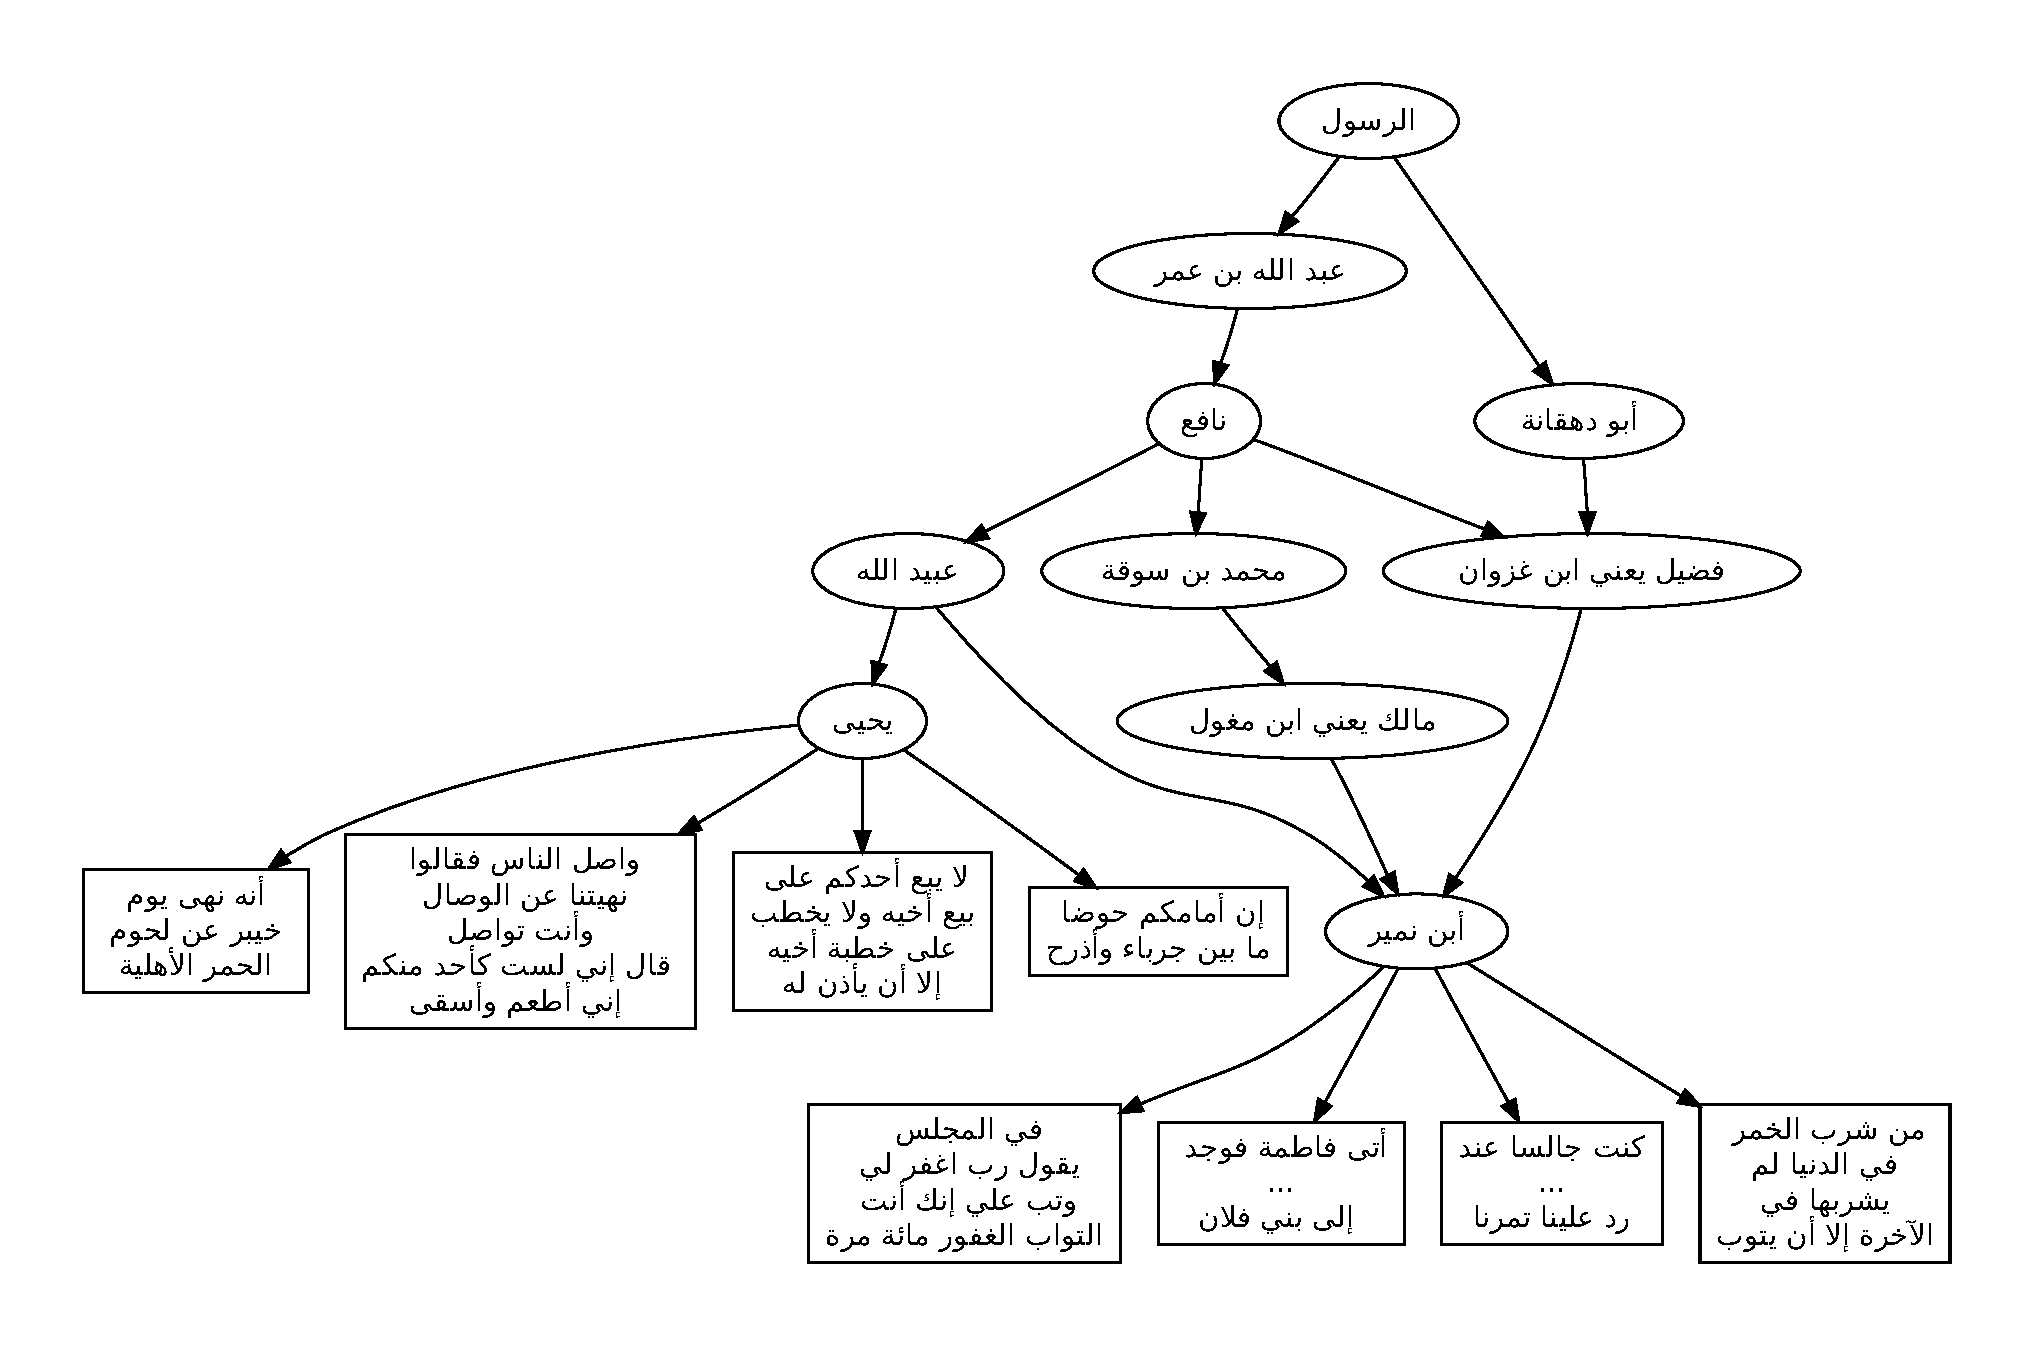
\includegraphics{figs/narrator_chain_output.pdf}}
\caption{Directed acyclic graph representing a partial order 
    relation between narrators extracted using ATSarf}
\label{f:narrators} 
}
\end{figure}

The directed acyclic graph (DAG) 
in Figure~\ref{f:narrators} shows a partial order relation (POR) 
between narrators.
We automatically extracted the POR from three books of hadith 
selected arbitrarily~\cite{IbnHanbal,AlKulayni,AlTousi}
\footnote{We obtained
  the digitized books from online sources such as 
  \href{http://www.yasoob.com/}{http://www.yasoob.com/} and 
  \href{http://www.al-eman.com/}{http://www.al-eman.com/}. }.
The nodes in boxes are the \RL{matn} of the hadith, 
and the other nodes are the narrators.
Given a set of chains of narrators similar to 
Figure~\ref{f:exhadith} we formed the DAG using graph algorithms 
that merged equal names in the chains. 
This partial order graph is instrumental to automate
localizing narrators in biography documents and
segmenting biography documents.

Given that a biography will discuss a narrator and mention
his professors and students,
we can segment the biographies with a graph coloring algorithm 
that traverses the text and colors the POR whenever
a name is found. 
We modify the color when we move in the graph 
far away from the last name we colored.

Once the biographies are analyzed, one can annotate
the POR with qualifiers of the narrators that reflect
their authenticity. 
One can also annotate the POR with the locations and 
the time they lived in. 
Then one can compute a time and location overlap
check to discover inconsistent narrations.
We can also perform several interesting checks using 
this POR on its own such as checking for the effect of
one narrator on the hadith literature. 

These preliminary results serve as a good proof of concept to our 
hypothesis. They also confirm that our approach performs better than 
currently existing techniques from Sakhr~\cite{Sak09},
Basis~\cite{Bas09} and open source 
tools~\cite{Col09,Otakar:07,Tim04}.

We find evidence in our current results that features 
of the Arabic language such as the hierarchical structure of
names can be used to simplify the morphological analysis
needed to extract the partial order graph. 
Publications about these results are pending acceptance in 
related NLP conferences. 

\subsection{Related work of principal investigators}

The Co-LPI, Rehab Duwairi, has several years of experience 
working on data mining for Arabic documents. 
She initially targeted Arabic text categorization where a 
data set of 1,000 documents was used to train and test 
classifiers~\cite{Duw06,Duw07}.
Word morphology comes to the surface when extracting the 
feature vectors of documents. 
In that work, words were stemmed before using them as features. 
Also, word frequency and inverted term frequency were used to 
quantify the importance of features. 

In a recent work, Duwairi, Refae and Khasawneh~\cite{Duw09}
have addressed text categorization again. 
This research investigated possible word forms that can be 
used to create feature vectors of documents in particular: 
original word, stem of the word, light-stem (shallow stemming) 
of the word, and word augmented with a list of synonyms. 
Therefore, every document is represented using four different 
feature vectors, the result revealed that light-stemming is the 
best representation as it preserves the meaning of the words 
and yet reduces the dimensions of feature vectors. 
The data set size was 15,000 documents that belong to three 
categories. 

The Co-Lead PI published extensively in the 
domain~\cite{Duw06, Duw07, Duw09}.
In recent research efforts, the CO-LPI is investigating 
keyphrase extraction fro Arabic documents.

The Lead PI worked in the area of software Arabization since 1996 
as he worked on developing Arabization modules for Windows NT 
and an Arabic string manipulation library~\cite{Zar96}. 
The Lead PI is also involved in working on an open source 
project that aims at comprehensive automation of authenticity 
checks against a corpus of hadith literature~\cite{Zar06}.
The Lead PI is leading an effort at AUB to introduce 
Computational Arabic in the curriculum of the ECE program. 
He is also leading a team of students in an effort to place 
the infrastructure needed for this project to start. 

The lead PI holds several approved patents and has several 
patents pending approval in the area of logic verification 
and synthesis.
The lead PI worked and published about relational logic and 
logic solvers applied to structured languages~\cite{seraICSE07,Zara05}

\section{Research design and methods}
\label{s:designmethods}

The specific aims of this project are:
\begin{itemize}
\item Build the CATARM framework while solving four interesting Arabic 
text minining case studies
  \begin{itemize}
  \item Hadith literature case study
  \item Security case study
  \item Network content case study
  \item Health case study
  \end{itemize}
\item Build and enhance a case-based morphological analyzer
\item Build an Arabic linguistic computational model (LCM)
\item Build entity and relation extractors
\item Build a query language 
  \begin{itemize}
  \item Build optimization modules that use the query to reduce the LCM
  \item Build a query solver that compiles all the components and run them 
  \end{itemize}
\item Build language independent LCM optimization modules
\item Add statistical, graph, and text manipulation algorithms
\item Build a visualization tool to showcase the results 
\end{itemize}

In the rest of this section, we will introduce Arabic text mining in 
details, then we will discuss the case studies in 
Sections~\ref{s:design:lit}--~\ref{s:design:med}. 
We will discuss the morphological analyzer in Section~\ref{s:design:ma}, 
the query language in Section~\ref{s:design:query}, and the linguistic
computational model in Section~\ref{s:design:lcm}.
In Section~\ref{s:design:method}, we will discuss our methodology
to build the components, optimize and reduce the LCM, build the
entity and relation extractors, solve the query, and visualize the 
results. 
Section~\ref{s:design:plan} will details the work plan and
justify the proposed budget.

\subsection{Arabic text mining}
\label{s:design:atm}

We see more and more Arabic documents such as texts,
books, publications, hospital and governmental records emerging 
every day.
Most of the newly generated documents are produced in digital 
textual form while also old paper documents are ported to digital 
form.
These documents include huge amounts of information that is 
qualitatively different than structured information such as that 
contained in database entries.
Text mining is the technology that automates the discovery of 
information in non structured text.

Text mining concerns the partitioning of text segments 
into classes,
the clustering of text segments,
the extraction of concepts and entities from text,
and the discovery and modeling of relations between text entities 
and classes.
Text mining techniques perform NLP to analyze text and perform 
IE to extract information into data structures.
Fundamental to IE are the named entity (NE) and the named entity 
relation (NER) extraction techniques which capture features from 
sentences and phrases.
A key challenge to NE and NER is that sentence structures and 
words are often ambiguous in natural languages.
%While research to address ambiguity in Latin languages is still 
%lagging behind~\cite{Red08},
%not much has been done to address NE and NER in the context of 
%the Arabic language.

IR tools are similar to a Google search 
engine where documents of interest are selected based on the 
relevance to a set of keywords of interest to the user.
NLP targets the automation of understanding human languages.
This task is the oldest and most difficult task in the artificial 
intelligence domain.
The main difficulty behind NLP comes from the ambiguity of 
natural languages~\cite{Osm08}.
While NLP techniques cannot deliver their final target yet, they 
can deliver analysis of sentences into nouns, verbs, 
and adjectives.
They can also narrow the meaning of a word or a phrase based on 
the context to one of its possible meanings.
Finally they can parse a sentence into a relation between the 
discovered entities using abstractions such as verb-name 
abstractions~\cite{Osm08}.

IE targets forming data structures and instances of these 
data structures out of a collection of documents.
IE tries to fit the output of IR and NLP to templates of 
interest to the user.
Data mining can be applied at the end on the output of the 
IE process to answer user queries about the input 
documents~\cite{JHa05}.


The application of text mining techniques to Arabic text documents 
will result in great benefits to many research fields such as 
Arabic literature,
Islamic studies, Hadith authentication, and Arabic history and 
culture in general.
Arabic text mining will also benefit sectors where Arabic text 
documents are key such as the security sector,
the government personal records,
the taxation department,
the health sector,
as well as the trading floor of a stock exchange.
 
%The difficulty of applying text mining techniques to Arabic text 
%documents lays in the absence of automated tools that understand 
%the unique features of the Arabic language.
%We will make use of an example to illustrate the process.
Given an Arabic text document we want a tool that can segment 
and isolate all names, dates, time of the day occurrences,
tool names, and locations as entities.
Then we want another tool to identify relations amongst 
these entities such as identities and orders.
We want another tool to look at the verbs and actions in 
the sentences and try to build relations between the identified 
entities based on these verbs.
If we were successful to do that,
we now want to order all entities associated with dates based 
on a chronological order.

An order between two entities can depend on 
their simple order of appearance in the document, their 
numerical values in case they happened to be numbers, or
the distance between them in case they were cities. 
The relations can also be more sophisticated and 
based on templates provided by users or by 
models extracted from training data sets. 

To do the above, 
we need tools that automatically differentiate between 
names, verbs, adjectives and other structures.
This is not a simple task with the Arabic language.
For example, Arabic grammar allows name-based sentences 
or sentences with no verbs \noTrNoVocRL{^gml ismiyT} .
Another unique feature is the possibility to have names in Arabic 
that express action such as noun verbs 
\noTrNoVocRL{ism f`l, f-a`l $\ldots$}.

In addition to these structural differences,
there are features in the Arabic language that need special 
treatment such as derivatives and stems 
\noTrNoVocRL{alm^staq-at w al^g_dwr}.
Simple primitive tasks such as comparing two strings need 
special attention in Arabic since each Arabic letter has 
four different forms depending on its position in the word; 
isolated form, start, middle and end of a word.
Arabic diacritics should also be ignored most of the time 
when comparing two strings.
We also need to build dictionary tools that associate words 
and phrases based on their meanings and their context.
Often time,
and depending on the application and the user of the tool,
we need to allow the user to assign meanings and semantics 
for patterns in the text.

We describe CATARM using four case studies and then move
to describe the different tools needed to build
CATARM.

\subsection{Hadith authentication case study}
\label{s:design:lit}

%\begin{figure}[tb]
\begin{figure}
\center{
\resizebox{.9\columnwidth}{!}
{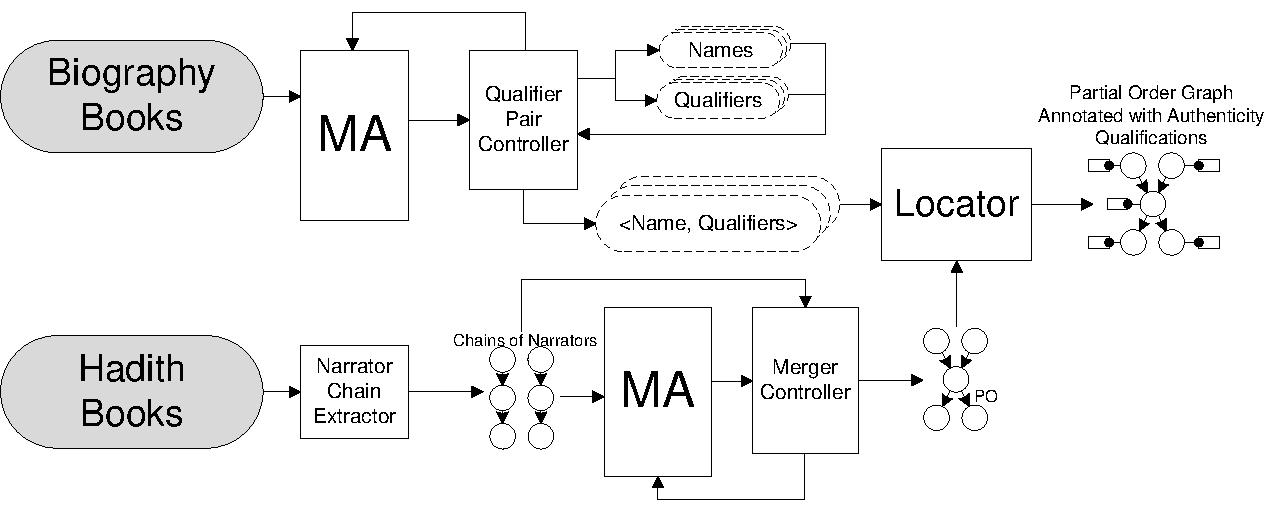
\includegraphics{figs/literature_case-study1.pdf}
} 
\caption{CATARM diagram for the hadith case study }
\label{f:literature}
}
\end{figure}

The diagram in Figure~\ref{f:literature} describes our 
high level vision for what the hadith case study
will look like in the CATARM framework. 
The boxes represent 
computational blocks provided by CATARM, 
ovals represent data blocks which are mainly the 
inputs and the outputs of the computational blocks. 
Dotted data blocks represent intermediate results,
and solid and shaded blocks represent the initial input 
and the final output respectively. 

The computational components can be direct CATARM components
or custom user components built from other CATARM components.
We feed the hadith books to a user Narrator Chain Extractor
component that we will discuss later in 
Section~\ref{s:design:method}. We  obtain a set of chains
of narrators that we feed to a morphological analyzer (MA) 
component controlled by a merger controller. 
The merger controller will look at the morphological analysis
of the narrator names and will decide to merge two narrators in 
one graph node in case they were morphologically equal. 
It will also give feedback to the MA component to stop the
analysis when a it reaches a satisfactory result.
We consider this graph as a partial order relation between 
narrators where a narrator precedes another narrator if 
he narrated from him. 

The biography books are fed to another MA unit controlled by 
a name and qualification pair controller that generates a 
map consisting of pairs of narrator names associated with 
qualifications. 
Then the graph of narrators and the narrator qualification map
are both processed through a locator component that computes
a graph coloring routine to color the graph of narrators. 
The color changes when two consecutive narrators are far away
from each other in the text. 
The locator then looks at connected subgraphs of the same color,
and finds a median node in each of them to be the narrator 
associated with the qualifiers of the color. 
Then the locator also annotates the narrator with the 
corresponding qualifications. 
The result is an annotated partial order graph of narrators
with authentication qualification annotations. 

\subsection{Security case study}
\label{s:design:sec}

%\begin{figure}[tb]
\begin{figure}
\center{
\resizebox{.9\columnwidth}{!}
{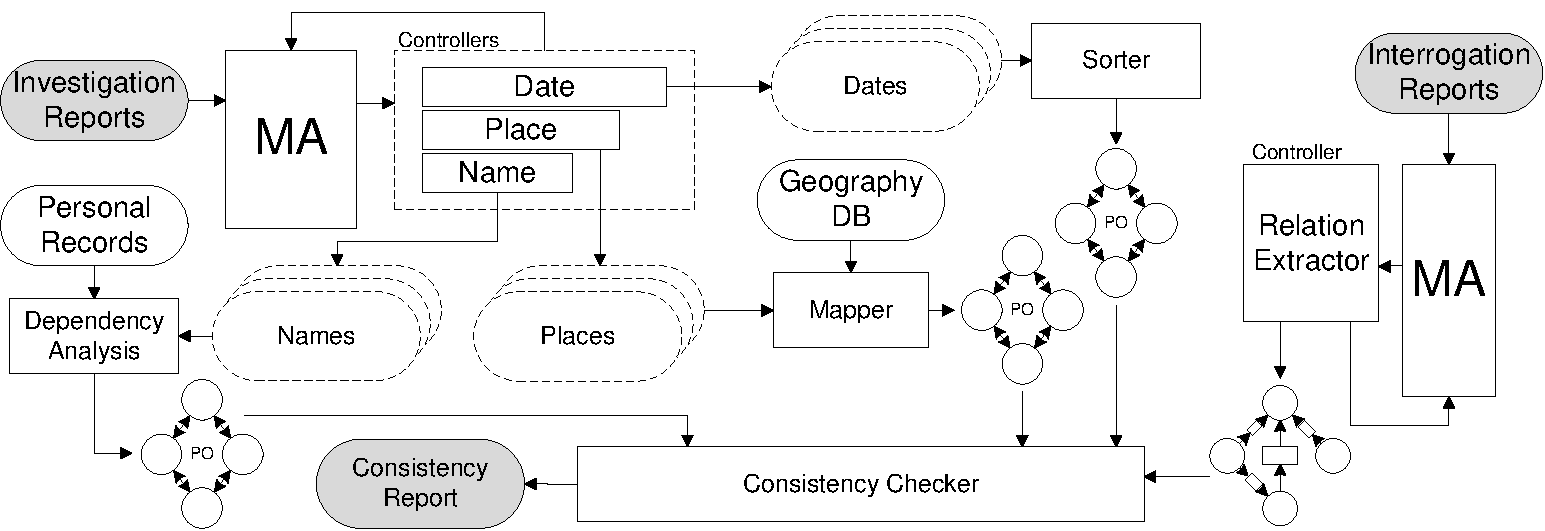
\includegraphics{figs/security_case-study.pdf}
}
\caption{CATARM diagram for the security case study}
\label{f:security}
}
\end{figure}


The diagram in Figure~\ref{f:security} describes our 
high level vision for what the solution of the 
security case study
will look like in the CATARM framework. 
The inputs are two separate sets of documents. 
The first set includes crime scene investigation reports, 
and the second set includes a 
interrogation reports with crime suspects as well as 
a database of previous interrogation reports. 
The CATARM system also takes as input a database of geographical
locations and a database of personal records. 
The aim is to check for inconsistencies in the interrogation
reports and to identify possible connections between the suspects
and the crime scene. 

A morphological analyzer with date, place, and name extraction controller extracts
names, dates and places from the investigation reports. 
We pass the dates to a sorting component to produce $G_D$ 
a partial order graph between the dates. 
We look up the names in the personal records database and find out
$G_N$ a family dependency graph between the names. 
We pass the places to a mapper that builds another $G_G$,
a graph relating the places using a geographical database. 

We pass the interrogation reports to an MA with a relation 
extraction controller that builds $G_R$. 
The graph $G_R$ relates the interrogated suspects
to each other, to places, and to dates based on a simple
neighborhood threshold computed using a statistical feature. 

We feed $G_D, G_F, G_G,$ and $G_R$   
to a consistency checker.
The consistency checker considers the three dimensions 
$N$ names, $G$ locations, and $D$ dates and projects $G_R$
over each one of them.
For each dimension $k$, it computes a local measure 
$\alpha_k$ of how much $G_R|_k$ simulates $G_k$. 
It flags the components in the graph where the accumulated 
measure $\alpha= \Sigma_{k\in\{D,N,G\}} \alpha_k$ is
below a threshold $\theta$ as inconsistent. 

As such reports contain sensitive information and our contacts
in the Lebanese security declined direct access, 
we will start the security case study by studying dummy documents that 
represent both interrogative and investigative types of documents. 
We collected a small amount (in the order of tens)
of similar documents published in the news in the last two years
from cases that were brought to public court or from high profile
cases that leaked to the media.
We will work on augmenting this collection further to have a large
enough set of reports (in the order of hundreds). 
We will mutate the entities in these documents and seed the mutated
set with relations we wish to discover and that are hard to discover
manually. 
Later on, we will use our contacts with the Lebanese and Qatari 
security authorities
to validate our system on their real data. 

\subsection{Network content case study}
\label{s:design:net}

Parental controls help parents allow their kids to benefit from the internet 
without fearing the danger of violent and obscene material. 
These controls partially rely on processing the content to detect and rate 
the target material. 
Control mechanisms for Arabic traffic as currently mostly manual. 
In this case study we will detect the bad content. 
Given a set of undesired internet content 
and a set of requests by internet users, 
CATARM can discover whether there is a relation between 
the requested documents and the undesired content and flag the 
requested document with strong enough relation. 

\subsection{Health case study}
\label{s:design:med}

Clinical reports contain diagnosis information, observations about 
patient progress, prescriptions, and patient response to prescribed 
medications. 
In countries, like Lebanon, where medical doctors graduate and specialize 
in several distinct practices around the world it is interesting to 
check for common practices and emerging trends to gain insight
about local and regional health and diagnosis features. 
It is also interesting to relate 
pharmaceutical 
records to clinical reports to check on 
market consistency and on self prescribed medicine 
practices.
Such a study can uncover serious tendencies in uncontrolled
pharmaceutical markets.
It can uncover what kind of sicknesses and what kind of medicines
are used sensitive medicines are used without 
appropriate medical supervision. 

We will work with our contacts at the American University
Hospital (AUH) at Beirut to analyze this data and relate it
to nearby pharmaceutical records. 

\subsection{CATARM components}
\label{s:design:components}

To do the above we need CATARM to provide us with several 
computational components such as a morphological analyzer, 
statistical tools, graph algorithms, and other computational
components. 
In the following we discuss the components needed for 
CATARM and we propose a methodology to 
use and extend existing tools, and develop new tools to
build the components of CATARM.

\subsection{Case-based morphological analyzer}
\label{s:design:ma}

Morphological analyzers for the Arabic language
such as Buckwalter~\cite{Buckwalter:02},
Beesley~\cite{Beesley:01}, SAMA~\cite{Kulick:10},
and ElixirFM~\cite{Otakar:07} take an Arabic word as input
and produce several valid morphological solutions for the word. 
Each solution is a sequence of morphemes that form the word.
Each morpheme is associated with several tags such as 
morphological, part of speech, grammar, and semantic tags. 
These analyzers are essential in several text analysis tools such 
as spell checkers as well as NLP frameworks~\cite{Col09}.
Other morphological analyzers such as 
Amira~\cite{Diab:07,Benajiba:07},
MAGEAD~\cite{Habash:05}, and MADA+TOKAN~\cite{Habash:09} 
use machine learning and support vector machines (SVM) 
to enhance the accuracy at the expense of efficiency.

The current use of morphological analyzers suffers from 
several problems. 
Analyzers that enumerate all possible partitions of a word
and match them against concatenative rules are computationally 
expensive. 
Analyzers that exhaustively enumerate all possible solutions 
for a word may hurt performance and may
not be necessary or appropriate in some case studies~\cite{Maamouri:10}. 
For example, the first solution may be the one needed and 
we may not need to list the rest of the solutions. 
A white space delimited token may have more than one word
as is the case with ``run-on words''.

We propose to make use of the current existing morphological
analyzers to build a flexible and more efficient
morphological analyzer. 
The analyzer will be an essential
component in the CATARM framework. 
It will be a case-based analyzer as it will make guided decisions
based on feedback from the NLP case study and it will prune
invalid solutions on the fly. 

Case-based analysis can guide the morphological analysis
to prune lots of the solutions and to bias the order of considered
decisions. 
For example, in the hadith literature case study presented above, 
amongst other things, we are interested in checking whether a 
word is a name.  
We can bias the order of considered decisions to consider the 
morphemes that can be names first. 
If one of them matches, we can ignore the rest of the solutions. 
In case a prefix is decided to be of a morphological category
that does not connect with a name, then we can just ignore
the analysis of the rest of the word. 
This is more efficient than generating all possible partitions
of the word, checking for morphological correctness of each 
partition, and then inspecting the part of speech tags of each
correct solution. 
We desire to build a morphological analyzer that allows a 
case-based controller to intervene at every single decision
without much overhead. 

\subsection{CATARM query language}
\label{s:design:query}

We propose the CATARM query language with a user friendly
visual representation similar to that in Figures~\ref{f:literature} and
~\ref{f:security}. 
The basic elements in the query language will be entities, relations
and tags similar to those reported by a morphological analyzer. 
The query language will also have connectives such as set operations, 
relational operations, 
scalar and Boolean arithmetic operations, 
statistical computations, graph algorithms, and text algorithms
form terms and predicates that specify the desired computation
by the user. 
We will specify the CATARM query language in a formal grammar.

\subsection{Arabic linguistic computational model }
\label{s:design:lcm}

Several techniques~\cite{AEL07,Ham07,Abd07,MEl03} 
preprocessed the Arabic text and then used known text 
mining techniques that tend to Latin text and queries
to solve classification, indexing, named entity 
extraction and other problems.
We think that these techniques do not make use 
of Arabic language specific features.

We think that we can discover such features by building
a linguistic computational model of the Arabic language
based on its formal grammar and formal morphology
as defined in several Arabic linguistic 
sources~\cite{Sha73,Abd00,Abd001}.
We will build our morphological analyzer on top 
of this linguistic model in addition to the current existing
concatenative-based analysis techniques. 

Let $L_q$ be the query language grammar, 
$L_A$ be the grammar that expresses the Arabic linguistic
computational model, and let $q$ be a user query.
We compute $\rho_q$, the grammar path that matches 
the query $q$ in $L_q$. 
We will explore methods that use $\rho_q$ to simplify 
$L_A$ before we start the morphological analysis. 
We think the possible simplifications that we can perform
here are Language specific as they will reflect the 
correspondence between the formal query language definition $L_q$, 
the usage patterns of $L_q$  by Arabic users, 
and $L_A$ the formal LCM for Arabic. 


\subsection{Methodology}
\label{s:design:method}

\begin{figure}
\center{
\resizebox{.5\columnwidth}{!}
{\input{figs/hadith.pdftex_t}
}
\caption{State-machine used to detect the chain of narrators}
\label{f:statemachine}
}
\end{figure}

{\bf Case-based morphological analyzer.~~}
We experimented with several morphological analyzers.
We think that using finite state machines for morphological analysis
can be implemented in a more efficient way compared to other 
approaches. 
For example the concatenative rules used in Buckwalter~\cite{Tim04}
can be encoded in three FSM with linear execution time using 
the trie~\cite{Aoe:89} data structure. 

The use of FSMs also suits our case-based approach. 
The controller can be a FSM machine on its own and its decision
will be another input into the internal morphological FSM structures. 
This also suits our choice of enriching the concatenative analysis
with a formal linguistic model that can also be encoded into FSMs. 
FSM can also be easily integrated with hidden Markov models (HMM)
extracted from the sets of documents the MA will consider. 

The state machine in Figure~\ref{f:statemachine} controls 
the concatenation based state machines of the morphological
analyzer.
The transitions are excited
by inputs from the morphological analyzer. 
A NAME label represents a proper name, 
an NRC label represents a narrator connector such as
\RL{`an} "on behalf of", \RL{qaal} "said", 
or one of their derivations. 
The IBN label corresponds to the word \RL{ibn} 
``the son of'' and represents a name connector.

The symbol $\tau_{\mbox{NMC}}$ is a threshold
that corresponds to the number of tolerated name connectors 
that may occur between two names. 
The symbol LIST$_{\mbox{NMC}}$ corresponds to the list 
of name connectors collected since the controller
started looping in the state NMC\_S. 
The symbol $\lambda_{\mbox{NMC}}$ is a parameter 
that corresponds to a relaxed tolerance measure that
the controller resorts to in case the words separating
two names were longer than $\tau_{\mbox{NMC}}$ but 
contained a name connector word such as IBN or NISBA.

The controller has four states that correspond to 
an abstract position in text relative to the next sanad. 
State TEXT\_S is the initial state and denotes that
the controller is outside the context of a sanad.
The controller moves to the state NAME\_S whenever
NAME is reported.
State NRC\_S means that the controller thinks it is in the context
of a narrator name after an NRC is reported.
State NMC\_S
indicates that the controller expects a name to appear within 
a tolerance threshold expressed by 
$\tau_{\mbox{NMC}}$ and $\lambda_{\mbox{NMC}}$.

Similarly, the NRC\_S state tolerates $\tau_{\mbox{NRC}}$ words 
before it gives up on its expectations. 

We reach the NAME\_S state only when a
valid NAME is detected and we leave when no more NAME's 
are detected. 
The NRC\_S state can only be reached if an NRC is detected.
NMC\_S can only be reached from a NAME\_S state.

The controller reports a valid chain of narrators when a 
sequence of names
connected by narrator connectors appears. 
It marks the beginning of the hadith with the beginning of the 
current sequence,
and marks the end of the hadith with the beginning of the next 
sequence. 
It also marks the chain of narrators as the sequence itself. 
The definition of input labels such as NAME and IBN depends on 
the morphological analyzer. 
We readily implemented the above approach and confirmed its 
accuracy and efficiency compared to existing morphological
analyzers. 

We will investigate enhancing our current case-based morphological
analyzer.
We will investigate methods to extend the internal structures 
of our analyzer to be able to represent a formal linguistic
computational model of the Arabic language. 

{\bf Linguistic computational model of Arabic.~~}
We think that a linguistic computational model for the Arabic
language will perform better in applications where
relations between Arabic text documents are involved. 
Such a model helps capture features unique and specific 
to the Arabic language and make use of that in the analysis.

ElixirFM~\cite{Otakar:07} builds on the lexicon
of the Buckwalter analyzer and the annotations of the 
Prague Arabic dependency databank to build a formal 
computational model of the Arabic language.
The model is a set of formulas and rules. 
ElixirFM uses the computational model in a functional
morphology framework that uses Haskell and functional
programming. 
The analyzer works by generating morphological trees of 
decisions and then uses a disambiguation decision procedure 
to annotate the trees with contextual elements. 

We will explore extracting our model from formal text book
definitions of the Arabic language~\cite{Abd00,Abd001} and seek
help from Arabic linguists to relax these formal rules to
allow common mistakes. 
We will encode the model in a grammar that we can synthesize
into an FSM and incorporate that with our current FSM 
morphological analyzer. 


{\bf User query language.~~}
In Figure~\ref{f:statemachine} we showed an FSM 
that controls the morphological analysis and generates a
list of chains of narrators out of hadith text.
We think that it is overwhelming to ask a user who is not 
versed in FSM and in computational sciences in general 
to design such a controller. 

The diagram in Figure~\ref{f:chain} depicts our vision of 
an equivalent query.
This query generates the list of chains by first passing the 
hadith text into the morphological analyzer which 
extracts names and their position in text. 
We iterate over the extracted names and compute the distance.
Whenever the distance is less than a threshold $\theta_1$
we add the word to a temporary chain of names. 
Otherwise, we execute a sequential block to 
{\bf 1.} tabulate the chain into a temporary table containing 
the list of chains. 
{\bf 2.} Create a new chain with the last element.
Finally, we filter those chains whose cardinality 
is less than some threshold  $\theta_2$.

This query can be saved to a library of computational components
and invoked directly in another query 
as we saw in Figure~\ref{f:literature}.

\begin{figure}
\center{
\resizebox{.9\columnwidth}{!}
{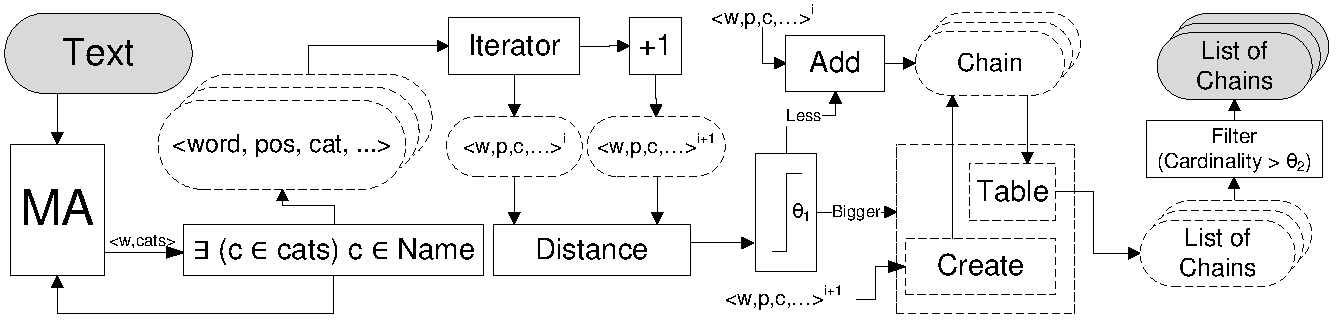
\includegraphics{figs/detailed_submachine.pdf}
}
\caption{CATARM detailed diagram for the chain of narrators extractor}
\label{f:chain}
}
\end{figure}

The CATARM query language will be expressed in a grammar 
where the atomic elements are user defined constants, or
entities and tags extracted by the morphological analyzer. 
The language will define terms, expressions, and predicates
using several connectives that express set operations, 
relational operations, Boolean operations, scalar operations, 
statistical tools, text algorithms, and graph algorithms. 
We need to provide a front end tool to support this query
language.

{\bf Simplify LCM based on the query.~~}
Given $L_q$ the query language, 
$L_A$ the Arabic linguistic
computational model, and  $q$ a user query
we compute $\rho_q$, the grammar path that matches 
the query $q$ in $L_q$. 
We plan to inspect methods to over-approximate 
the morphemes and the transitions in $L_A$ 
that can be satisfied by morphemes and transitions
in $\rho_q$. 
This can simplify the number of states we need to 
look at under $L_A$. 

This task is not trivial though, since $\rho_q$ may contain
states and transitions that are not always morphemes and 
transitions between morphemes. 
We will consider a hierarchical methodology that follows 
the hierarchical structure of the Arabic language expressed
in $L_A$. 
Consider $\Phi$ the state machine representing the grammar 
rules for $L_A$ and consider $\phi$ the parse graph 
representing $\rho_q$, in particular consider the atomic nodes 
representing lexical entries in $\phi$. 
Consider $S$ to be the set of states in $\Phi$ that 
correspond to these nodes. 
Consider simplifying $\Phi$ using techniques that remove 
states and transitions that do not lead to $S$. 
An optimal reduction requires expensive reachability 
analysis, however, we can apply simpler reductions such 
as structural cone of influence reduction,
constant propagation reduction that overapproximate
reachability analysis. 
%For example, we may consider sets of connected states in $\rho_q$ 
%containing a single morpheme as a state in one hierarchy level 
%in $L_A$.
We will perform this simplification before starting the 
morphological analysis since we already have to analyze
the query $q$ and compute $\rho_q$ before we start
the analysis. 

{\bf Simplify LCM and MA based on documents.~~}
We will analyze the set of input documents given to a
morphological analyzer component and use the analysis
to further improve the morphological analysis. 
We will extract statistical features from these documents 
to help order the solutions considered by the analyzer
and consider the most probable first. 

We will consider the use of HMM~\cite{JanHMM06}
models built on the fly while processing the documents.
A high level HMM model of the document builds an HMM state
model where the HMM states are morphemes or partial 
morphemes and the HMM edges represent transitions between
the HMM states. 
The HMM edges are labeled with weights that reflect the
We will look at building a correspondence between 
the HMM model and the LCM and then simplify the 
LCM where the aggregated probabilities happen to be
below a certain threshold. 
The work in~\cite{JanHMM06} uses a similar approach
to correspond English text to tags corresponding to the 
Unified Medical Language System (UMLS).

We will also consider the use of
latent semantic indexing~\cite{LSI89} techniques. 
We are considering these two techniques as they are 
both language independent and can both be computed and
adapted on the fly.

{\bf Entity and relational extractor.~~}
We will build a set of entity and relational extractors. 
The entities can be proper names, dates, locations,
and qualification adjectives. 
We will explore the use of pairing techniques to establish 
relations between the extracted entities.
The relations will form graphs as in the case studies presented
so far. The nodes represent the entities and the previously 
extracted relations and the edges represent the newly discovered 
relations.

The entity and relational extraction components 
may take as input a template for an expected relation and 
may return a graph that describes whether and where 
this relation exists between the subject documents.

We will need to augment the tags in the lexicons of the 
morphological analyzer to allow for better entity and relational
extractors. 
We plan to make use of existing annotated tree banks and of
modern Arabic dictionaries to do that. 

{\bf Statistical components.~~}
We will make use and build statistical components that can be used
in CATARM. 
We will need statistical components to rank solutions, compute 
probable decisions, estimating good thresholds. 

{\bf Graph algorithms.~~}
The relations extracted from the text documents will often 
be expressed in terms of graphs.
We will need textbook graph algorithms such as traversals, 
topological sorts, spanning trees, strongly connected 
components, minimum flow  and other algorithms.
For example, in the hadith literature case study, the discovery
of articulation vertices may point to important narrators 
who may have an insignificant number of narrations 
but still connect narrator communities.

{\bf Query solver.~~}
The query solver considers query expressions and resolves them 
into matching text and relations. 
The solver returns and ranks approximate matches.
That is if a three entities out of four required in a relation are
found, the solution is still worth reporting. 

The solver passes the query to a front end that builds
a parse graph of the query. 
It uses the parse graph to simplify the LCM and the MA
as discussed before. 
Then it traverses the resulting parse graph. 
When the solver meets an atomic element of the query, 
it will call the morphological analyzer to compute 
morphological matches to the atomic element.
When the solver meets an operation of the query, 
it will call the corresponding computational component 
and passes to it the solutions computed so far from children
nodes. 
The solver will use existing off the shelf constraint solvers 
and set theory satisfiability solvers to address the queries. 
The solver may make use of existing 
propositional~\cite{MiniSAT04} or
higher order logic~\cite{Z308} solvers if needed. 
These solvers can solve satisfiability questions.

We explain the ranking aspect of the solver with a simple
example. 
Consider $q$ the parse graph of a query with $n$ nodes where 
each node corresponds to either a detected entity or
to an operation that can be computed with one of CATARM components. 
We define the rank of a solution to be the ratio of  the 
satisfied nodes in $q$ over the possible satisfied
nodes in $q$. 

%We will explore the feasibility and utility 
%of extracting a necessary set of 
%constraints from the query and answering that with an off-the-shelf
%logic solver. 

{\bf Case studies.~~}
We will work on developing the necessary components to complete 
the solution for the hadith literature  case study. 
We will also work on the security, health and network traffic case studies.
While working on the case studies, we will add the components
we build to our library of components. 
This will enrich CATARM with a useful set of computational 
components. 

{\bf Visualization.~~}
We will build a visualization tool that allows fast 
and guided inspection and correction mechanism. 
The CATARM visualization aid will be a tag and relation color
sensitive browser.
The interface will allow a fast and guided inspection and 
correction mechanism.

\subsection{Research team}

The team will be formed by the two main PIs, Dr. Fadi Zaraket (LPI)
and Dr. Rehab Duwairi (Co-LPI) and three research assistants.
Currently the LPI is working with one research assistant 
and two senior students on an Arabic morphological analyzer. 

The LPI offers a course on computational Arabic attended
by excellent senior and graduate students at AUB. 
Once funded, the team can be directly formed and work can start
with readily productive team members. 

\subsection{Work plan}
\label{s:design:plan}


%\begin{table}[bt]
\begin{table}[bt]
\centering
\caption{Three year quarter based work plan.}
%\begin{tabular}{|p{1.5cm}||c|c||c|c||c|c|} \hline
%\begin{tabular}{lp{.2cm}ccp{.2cm}ccp{.2cm}cc} %\cline{2-10}
\small
\begin{tabular}{lp{.1cm}ccccp{.1cm}ccccp{.1cm}cccc} \\
& & \multicolumn{4}{c}{Year 1} & & \multicolumn{4}{c}{Year 2} & & \multicolumn{4}{c}{Year 3} \\ \cline{3-6} \cline{8-11} \cline{13-16} %\\
    %\cline{2-13} \\ 
& & Q1 & Q2 & Q3 & Q4 & & Q1 & Q2 & Q3 & Q4 & & Q1 & Q2 & Q3 & Q4 \\ \bottomrule

Case based & & 
W & W & W & E & & E & E & E & E & & E & E & E & E \\ 
morphological analyzer & & 
 &  & D & DM & &   & M & M & M & & M & M & M & M \\  \hline

\multirow{2}{*}{Arabic LCM} & & 
P & W & W & W & & W & E & E & E & & E & E & E & E \\ 
& & 
 &  &  &  & & D & DM & M & M & & M & M & M & M \\ \hline

\multirow{2}{*}{Query language} & & 
P & P & W & W & & W & W & E & E & & E & E & E & E \\ 
& & 
  &  &  &  & &  & D & DM & M & & M & M & M & M \\ \hline

Language & & 
P & P & P & W & & W & W & W & W & & E & W & W & W \\ 
optimizations & & 
 &  &  &  & &  &  &  & D & & DM & M & M & D \\ \hline

Data  & & 
P & P & P & W & & W & W & W & W & & E & W & W & W \\ 
optimizations & & 
 &  &  &  & &  &  &  & D & & DM & M & M & D \\ \hline

\multirow{2}{*}{E/R extractors} & & 
W & W & W &  & & E & E & E & W & & W & W &  & E \\ 
& & 
 &  & D & DM & & M & M & M & M & & M & D & DM & M \\ \hline

Statistical & & 
W & W & W & E & & WE & WE & WE & E & & WE & WE & WE & WE \\ 
components & & 
 &  & D & DM & & M & M & M & DM & & M & M & M & M \\ \hline

Graph  & & 
W & W & W & E & & WE & WE & WE & E & & WE & WE & WE & WE \\ 
components & & 
 &  & D & DM & & M & M & M & DM & & M & M & M & M \\ \hline

\multirow{2}{*}{Query solver} & & 
P & P & W & W & & W & W & W & E & & E & E & E & E \\ 
& & 
 &  &  &  & &  &  & D & DM & & M & M & DM & M \\ \hline

\multirow{2}{*}{Case studies} & & 
W & W & W & W & & W & W & W & W & & W & W & WE & E \\ 
& & 
 &  & D$^1$ &  & &  &  & D$^2$ &  & &  & D$^3$ & D$^4$ M & M \\ \hline

\multirow{2}{*}{Visualization} & & 
P & W & W & W & & E & E & E & E & & E & E & E & E \\ 
& & 
 &  &  & D & & M & M & M & M & & M & M & M & M \\ \hline

\multirow{2}{*}{Integration} & & 
P & W & W & W & & W & W & W & W & & W & W & W & E \\ 
& & 
 &  &  & D & & D & D & D & D & & D & D & D & M \\  \hline

Validation & & 
W & W & W & W & & W & W & W & W & & W & W & W & W \\  \bottomrule
        %\cline{2-13} \\
\end{tabular}
\normalsize
\label{t:workplan}
\end{table}

We will follow an eXtreme Programming 
methodology in the process of building CATARM.
This means that we will define refined incremental items of 
work that allows for more frequent deliverables. 
This also means that the code base will always be subject
to maintenance and refactoring to enhance reuse and 
increase productivity. 
While a item is delivered, it will still be subject to work,
enhancements, and maintenance. 

We detailed an aggressive work plan in Table~\ref{t:workplan}. 
The plan spans over three years each with four quarters. 
The row headers describe work items, and the column headers
describe quarters in the corresponding year of the project.
The legends {\bf P, W, D, M, } 
and {\bf E} 
describe the type of activity taking place 
and stand for 
{\bf P:} {\em plan}, 
{\bf W:} {\em work }, 
{\bf D:} {\em deliver}, 
{\bf M:}  {\em maintain}, 
and 
{\bf E: } {\em enhance} respectively. 

The $1,2,3,$ and $4$
superscripts of the deliverables in the 
row of case studies refer to the four 
case studies described in the proposal. 

Work can happen on all items in parallel. 
Planing and research work can start on items that depend
on other items. 
For example, the LCM optimization items will be under 
active planing and do not need to be totally idle 
while the LCM is being built. 
That will allow better chances to build the LCM data structures
in a flexible way that requires less modifications if any
when the optimizations take place. 

That said, we describe the dependency of the items on 
each other as follows. 
The work on language optimizations and data optimizations 
depend on the Arabic LCM item. 
The work on language optimizations depends on the design
of the query language as well. 
The work on the query solver depends on the design of the 
query language. 
The entity and relation extractors depend on the morphological 
analyzer. 
However, they can start since we have already
developed an working analyzer as a preliminary step. 
The rest of the items can all work in parallel. 

We will use open source tools, libraries, and frameworks to 
build our componenets.
We will build on existing open source programming and text 
mining tools as well as open source Arabic text analysis tools 
based on NLP such as MADA+TOKAN~\cite{Rot08}, 
NEMLAR~\cite{RAl09}, and IJAES~\cite{Int09}.

We will use a dokuwiki based website~\cite{Dok09} 
to document the progress online and will use 
subversion~\cite{Sub09} as a source control tool.
 
The Lead PI will conduct biweekly meetings to track progress 
on the project.
The team will maintain a dokuwiki based website to continuously 
post updates on the progress of the project.


\subsection{Budget items}

In the following we list the budget items. 
Monetary values are provided in more details on the QNRF 
submission website. 

\begin{itemize}
\item One research assistant at QU
\item Two research assistants at AUB, one of them will 
work partially from QU. 
\item Two month salary per year for the Co-LPI
\item Two month salary per year for the LPI
\item One course buyout per year for the Co-LPI
\item Two weeks consultant for the second and the third years
\item Licensing and membership fees to acquire digital libraries and corpora
\item High performance computer and storage devices
\item One conference for each PI per year
\item One conference for one RA from QU per year
\item One conference for one RA from AUB per year
\item Site visit to AUB 
\item Site visit to QU 
\item Other miscellaneous items
\end{itemize}


\section{Anticipated results and evaluation criteria}
\label{s:results}

We anticipate that the research will lead to the production of 
CATARM, an Arabic text analysis framework that allows relational 
queries between Arabic text documents.
The components of the framework are listed and discussed
in details in Section~\ref{s:designmethods}.
In the following we will discuss what to anticipate and 
how to evaluate the different components of CATARM. 

\subsection{Case-based morphological analyzer} 

We will deliver a case-based morphological analyzer. 
The analyzer will be compared to other available analyzers such as
Buckwalter~\cite{Tim04} and ElixirFM~\cite{Otakar:07} in terms
of accuracy and efficiency of analysis.
We will adopt two comparison methodologies. 
First, we will compare the analyzers in an exhaustive analysis mode
which is the only way current analyzers perform. 
Second, we will compare the analyzers under several case-studies
and show how a case-based morphological analyzer can benefit
from case-based optimizations.

\subsection{Linguistic computational model for Arabic}

We will build a linguistic computational model for Arabic 
based on an understanding of the formal Arabic grammar 
and on an abstraction of the current existing concatenation
based lexicons.
We will compare our LCM with that of ElixirGM~\cite{Otakar:07}.
We will study how much such a model can affect the analysis
in terms of accuracy and efficiency as well. 

\subsection{User query language}

We will build a query language for relational Arabic text mining 
and a front-end to compile a user query into an optimized
computation. 
We will check how user friendly and how expressive the language is.
We will compare our query language with the sophisticated 
interface of the MADA+TOKAN toolkit~\cite{Habash:09}.
We will look for other attempts to formalize Arabic text 
mining queries and we will also compare against 
formal text mining queries from other text mining domains such
as the gene ontology domain~\cite{GeneOntology10},

\subsection{Optimizations}

We will develop and evaluate our two optimization methodologies
and look for other optimizations. 
First we will use language specific features based on the 
LCM of Arabic, the grammar of the query language, and 
the Arabic query provided by the user to simplify 
the LCM and the morphological analysis. 
Second we will look at language independent techniques
such as HMM and LSI models extracted from the 
text documents and use that to simplify the analysis. 
We will perform the analysis with and without the optimizations
and compare the results in terms of accuracy and efficiency. 

%\subsection{ Entity and relational extractors}
\subsection{CATARM and case studies }

We will evaluate CATARM against the case studies
that we discussed in Section~\ref{s:designmethods}
and that are listed below. 
\begin{enumerate}
\item Hadith literature
\item Security
\item Health
\item Network content
\end{enumerate}

We anticipate CATARM to be able to successfully solve all the case
studies with reasonable computational resources available to the 
average user. 
We will also generalize the components we will develop to solve
the case studies into a library of components that can be used
in other case studies. 

\subsection{External evaluation }

The team will seek the assistance and help of an independent 
consultant in the middle of the second and third years of 
the duration of the project to evaluate and validate the results.

\section{Strategy for project continuation}
\label{s:continue}

If granted, this project will initiate a long term
research relationship between Qatar University
and the American University of Beirut. 
Once completed, the Arabic text analysis framework will be 
an open source contribution and developers from the Arabic 
world in the open source community are expected to join 
efforts to keep it going.
Furthermore, the Arabic text analysis framework 
can sustain itself by charging on support or expert use.

The framework or service on the framework can easily be 
commercialized to tend to the security, health, insurance, market,
news, media, or literature business sectors.
 
The area of Arabic text analysis will be a research area for 
a long time as NLP is one of the most complex computational 
problems.
The Arabic text analysis framework will be used by NLP 
researchers in the Arabic language field and those are 
expected to maintain and advance the framework.

\subsection{Future work}

The completion of the CATARM framework will result in a 
significant contribution to the research community of 
NLP in general and Arabic Analysis in particular. 
The CATARM framework will act as vehicle to enhance and advance 
research in the area. 
We look forward for additional contributions to the field 
such as the following.
\begin{itemize}
\item We will explore developing and integrating vocalization
techniques. 
Vocalization techniques assign diacritics to unvocalized text. 
The prerequisites of a successful vocalizer are the accuracy of 
the morphological analyzer in addition to grammatical analyzers. 
\item We will explore the use of CATARM with more case studies
such as market analysis and opinion mining.
\item We will explore augmenting the lexicon of the
morphological analyzer with useful categorization and entity 
tags that reflect semantical meanings. 
These modifications would give CATARM additional capabilities in 
terms of allowing users to extract and use a greater variety of 
entities when building queries. 
The feedback of experts in the field of Arabic linguistics can 
continually add accuracy to the morphological solutions.  
\item We will explore further optimization techniques
that can help simplify and the analysis. 
\item We will explore generalizing our results to languages 
that resemble the Arabic language. 
Some Semitic languages, such as the Amharic, Cyrillic, and Hebrew,
share common features with the Arabic 
language. Some other languages are written using the 
Arabic script like Persian, Kurdish, Urdu, and Pashto. 
\item We will also investigate the case-based approach with
Latin languages and check how that compares with current techniques
in terms of accuracy and efficiency.
\item We will maintain CATARM and provide support to users and 
researchers of CATARM.
\end{itemize}


\section{Plans for disseminating research results}
\label{s:dissem}

The team will publish the results of the research in the form 
of refereed conference and journal papers as well as tool papers 
addressing each of the tools. 
The team will also hold workshops to educate possible users on the 
tools once the tools are available.
Graduate students such as Masters and PhD students are examplary t
target audience for such workshops.
The Arabic text analysis framework will be partially based on 
existing work in the open source domain and will thus be available 
as an open source tool. 
Interested researchers and users will be able to download the 
tools for free and use them for non-profit non-commercial 
purposes.  

\pagebreak
%\bibliography{adnan_refs}
%\bibliographystyle{ieeetr}
\bibliographystyle{abbrvnat}
%\bibliographystyle{ieeetr}
{\small
\bibliography{fzAr}  
}


\end{document}
